\chapter{Testing}

\section{Overall Approach to Testing}

High coverage on service layer, but more concerned with feature coverage rather than line coverage in general. Automate as much of the testing as is feasible so it can run as part of the CI build 

\section{Automated Testing}

For the purposes of automated testing, a separate database was used. The database would be completely recreated for the start of each run of the test suite and dropped at the end. Prior to the tests running, the database would be seeded with test data that is similar to the real world data expected in the production database. By using this method the tests would more closely mirror the real world behaviours of the system and each run could be insulated from the data changes made in previous runs.

A Continuous Integration(CI) system was used in order to facilitate the convenient and regular running of all automated tests in the project. The CI system would build the project from source each time a commit was made into the version control repository. As part of this build process the full test suite would be run. Any issues encountered during this process, from compilation errors to test failures, would result in the build being rejected by the CI system. 

\subsection{Unit Tests}



\subsection{Integration Testing}

Integration testing for this project was achieved through testing of the MVC controller classes. The goal behind these tests was to make requests to the various available routes within the system and verify that the correct results are returned. 

% !TODO discuss the loading of 'realish' test data via data.sql :
%  Like the unit testing, integration testing makes use of the test data defined in the data.sql file which is pre-loaded by hibernate into the test database prior to test execution.

\lstjava
\lstinputlisting[label=simpleIntegration,caption=Simple integration test example]{sourceCode/mySnippets/testing/testShowPlants.java}


\subsection{User Interface Testing}

\subsection{Stress and Performance Testing}

Performance and stress testing was carried out through the use of Apache Jmeter\cite{_jmeter}, an open source Java application built to measure site and application performance under controlled loads. Jmeter enables the simulation of a number of concurrent users accessing a given site, these simulated agents follow a defined sequence of actions as specified in the test script. Unless otherwise stated the tests run with ten concurrent agents and the tests are repeated thirty times in order to smooth out any outliers in the data.

The tests were all carried out against the project hosted on the remote server provided by Ibers. The machine used to run the Jmeter scripts is a powerful desktop machine using a recent generation of Intel i7 processor featuring 4 cores and able to process 8 concurrent threads. It is necessary that the test machine be connected to the Aberystwyth University VPN in order to reach the target server although the impact of the extra overhead appears minimal and is considered for the sake of comparing results. Although the ten concurrent users may seem low, the throughput on average is over 100 requests per second when run from the test machine which is significantly more than ten real users would be able to generate.

For the purposes of this project Jmeter was used to assess whether pages in the site would load within defined time limits and whether implementation decisions have an adverse effect on performance. In general the goal was to have pages served within 300ms with a hard limit of 1000ms, or one second, although this does not include image load times. A target of 300ms is well under the 1 second limit for keeping a users flow of though as identified as part of a study conducted by Nielsen \cite{responseTimes}. Running the tests regularly could also help highlight issues that may not be uncovered under other forms of testing such as intermittent problems that could result in request errors that would be difficult to reproduce otherwise.


General results as output by Jmeter are included in figure~\ref{fig:jmeter_with_data} for an experiment which has been initialised with data. The initialisation is an important distinction because the amount of experiment data significantly affects the initial page response time for the Graphs page, other pages are affected somewhat but to a much lesser degree. Figure~\ref{fig:jmeter_no_data} displays the results of running the same test without the data having been added to the experiment and it's clear to see the effect on the load time for the Graphs page. Having these results available during development informed some of the design choices within the Graph page such as having the graphs themselves and any plant objects loaded via Ajax following user interaction as opposed to being populated into the page on load.
\begin{figure}[H]
    \centering
    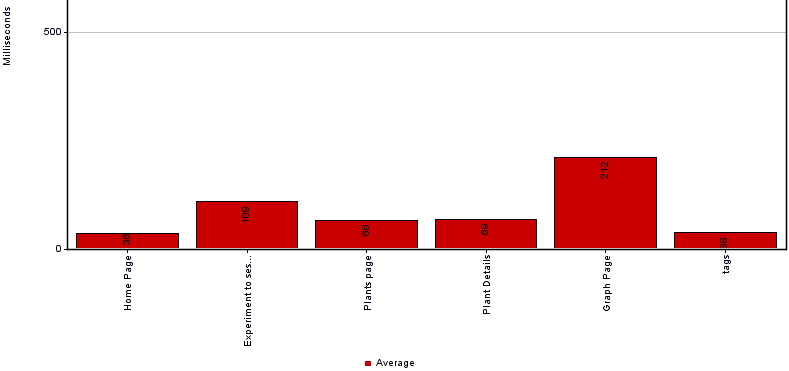
\includegraphics[width=\textwidth]{images/testing/jmeter_final_crop}
    \caption{Visulisation of Jmeter test result of a fully initialised experiment}
    \label{fig:jmeter_with_data}
\end{figure} 

\begin{figure}[H]
    \centering
    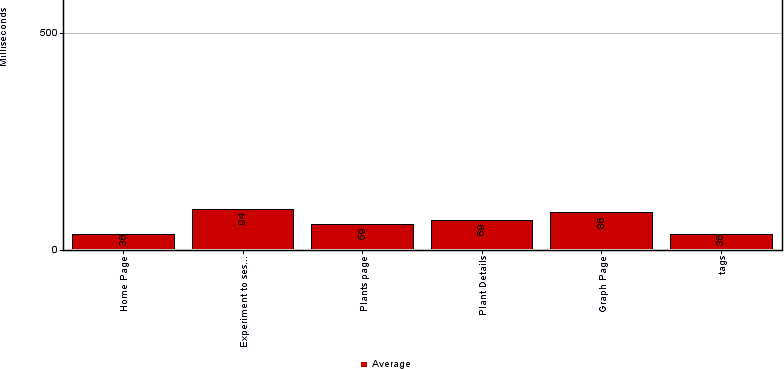
\includegraphics[width=\textwidth]{images/testing/jmeter_no_data_crop}
    \caption{Visulisation of Jmeter test result of a partially initialised experiment}
    \label{fig:jmeter_no_data}
\end{figure} 

The effect of choosing pagination defaults for the plants and plant detail pages could also be measured although in the case of pagination the real limiting factor is the bandwidth and render time required. However, the effect on request time and loading on the server could be seen and monitored for any potential issues.



\section{Manual Testing}
For areas of the system where automated testing was impractical or insufficient to verify results, a manual approach was taken and test tables used to verify functionality is as expected. 

\subsection{Admin Page Test Table}
Much of the functionality on the Admin page relies on an active network connection to the NPPC data repository and as such is unsuitable for automated testing. There was no feasible way to establish a connection between the continous integration server and the NPPC data repository therefore the manual verification of functionality is necessary.
\begin{table}[H]
\centering
\begin{tabular}{ | p{4cm} | p{4cm} |p{4cm} | p{1cm} | }
\hline
	\textbf{Test} & \textbf{Input} & \textbf{Expected Output} & \textbf{Pass} \\ \hline
	Attempt to access admin area without login & Go to /admin without login & Redirected to administrator login page & \checkmark \\ \hline
	Attempt to access admin area with correct login & Go to /admin with login & Admin is page is displayed & \checkmark \\ \hline
	Attempt admin login with incorrect credentials & Submit admin login form with incorrect credentials & Error displayed to user. & \checkmark \\ \hline
	Admin log out & Click logout button from admin page & Redirect to home page and authorisation cleared from session & \checkmark \\ \hline
	Initialise Experiment & Click initialise button for uninitialised experiment & Experiment begins initialising - plants are created & \checkmark \\ \hline
	Update experiment & Click Update button on initialised experiment & Experiment begins update, plants are updated or created & \checkmark \\ \hline
	Import data with valid csv & Click Init Data button on initialised experiment & Data is imported from csv & \checkmark \\ \hline
	Import data with invalid csv & Click Init Data button on initialised experiment & Invalid csv data is ignored & \checkmark \\ \hline
	Delete data & Click delete data on experiment & Data is deleted from the experiment & \checkmark \\ \hline
	Delete plants & Click delete plants button on experiment & Plant data and images are deleted & \checkmark \\ \hline
\end{tabular}
\caption{Test Table for Admin page functionality}
\label{test_table_admin}
\end{table}
\subsection{Graph Page Test Table}
Although most of the functionality within the Graph page is verified via automated testing, certain aspects require visual verification and as such a manual approach is taken to verify functionality within the page.
\begin{table}[H]
\centering
\begin{tabular}{ | p{4cm} | p{4cm} |p{4cm} | p{1cm} | }
\hline
	Test & Input & Expected Output & Pass \\ \hline
	Test view graphs with no experiment & Go to /graphs with no selected experiment & No data' page is show with back button & \checkmark \\ \hline
	Test view graphs with experiment that has no  data & Go to /graphs with experiment in session that has no data & No data' page is show with back button & \checkmark \\ \hline
	Test view graphs with experiment that has data & Go to /graphs with experiment in session that has data & Graph page is shown with graph creation options & \checkmark \\ \hline
	Test create graph & Click create graph button on /graphs page & A graph is displayed in the page with selected axis attributes & \checkmark \\ \hline
	Test box plot & Select 'Box' and create graph & Nodes in the graph are represented as box plots & \checkmark \\ \hline
	Test scatter plot & Select 'Scatter' and create graph & Nodes in the graph are represented as scatter plot & \checkmark \\ \hline
	Test swap axis & Click swap axis button & Selected axis attributes are swapped, x value becomes y value and vice versa & \checkmark \\ \hline
	Test plant results on graph node click & Click on or near a node in the graph & A  clickable list of plants corresponding to the values of the clicked node appear in the page & \checkmark \\ \hline
	Test click result plant & Click on a plant link generated as result of clicking on a graph node & User is redirected to the detail page for the clicked plant link & \checkmark \\ \hline
\end{tabular}
\caption{Test Table for Graph page functionality}
\label{test_table_graph}
\end{table}


\section{User Testing}